% This file should contain a short summary of the aerodynamic analysis tool and models

% Summarize the physics
To model the aerostructural performance of the wing, an open-source tool for preliminary sizing of aircraft wings called OpenAeroStruct~\cite{Jasa2018a} was selected.
OpenAeroStruct uses a vortex lattice method coupled with a 6-degree-of-freedom-per-node finite element model to analyze the aerostructural properties of aircraft wings.
These inexpensive physics-based methods enable inexpensive exploration of the wing design space which is valuable for conceptual level design studies.
Furthermore, OpenAeroStruct can be used to investigate both conventional and non-conventional wings as the physics-based analyses are not dependent on empirical  information from existing planes.
Lastly, OpenAeroStruct provides inexpensive derivatives for all outputs of the aerostructural analyses, which facilitates integration into multidisciplinary gradient-based optimization environments.

% Describe the model used by this tool that was developed for the tiltwing plane
Using OpenAeroStruct, a model was constructed to represent the wing of the tiltwing vehicle concept under consideration in this study.
The initial overall geometry (wingspan and root chord) were obtained from Johnson et al~\cite{johnson2018concept} with other aerostructural wing properties assumed based on similarly sized aircraft.
The relevant values for these parameters which were used in this study are listed in Table~\ref{t:aerostruct_wing}.
In addition to these parameters, a NACA 0015 symmetric airfoil was assumed for the wingbox cross-section, with this section occupies from 10\% to 70\% chord for the entire wing span.
The wing was also assumed to be constructed from Aluminum 2024 for the lower skin and spars and Aluminum 7075 for the upper skin with a safety factor of 1.5 applied on the yield strength of the wingbox material.
Finally, two point masses were included on each half-wing to account for the loading due to the engines and propellers with the magnitude of these masses coming from the upstream propulsion sizing analyses.
A three-view and isometric view of the aerostructural wing model including the approximate locations of the engines are shown in Fig.~\ref{f:OAS_wing}.

% Revise this table based on the actual optimization completed
\begin{table}[!htb]
 \normalsize
 \begin{center}
  \caption{Aerostructural Wing Properties.}
  \label{t:aerostruct_wing}
    \begin{tabular}{ l r l }
        \hline
        \textbf{Design parameter} & \textbf{Value} & \textbf{Units} \\
        \hline
        Wingspan & 52.50 & feet \\
        Root chord & 4.56 & feet \\
        Elastic modulus & 73.1 & GPa \\
        Shear modulus & 27.5 & GPa \\
        Yield strength (lower skin and spars) & 324 & MPa \\
        Yield strength (upper skin) & 503 & MPa \\
        Yield safety factor & 1.5 & -- \\
        Wingbox material density & 2810 & $\text{kg}/\text{m}^3$ \\
        \hline
    \end{tabular}
 \end{center}
\end{table}

\begin{figure}[h]
\begin{center}
 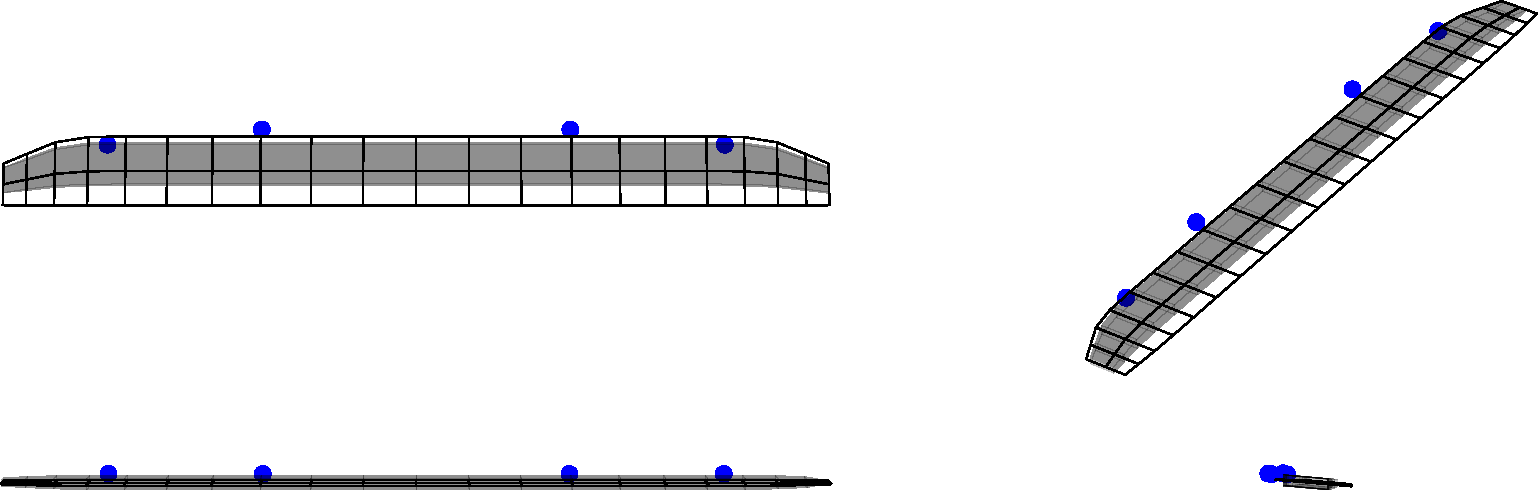
\includegraphics[width=1.0\textwidth]{../Images/aerostruct_wing}
 \caption{Three-View and Isometric View of the Aerostructural Wing Model with the Engine Point Masses Shown in Blue.}
 \label{f:OAS_wing}
\end{center}
\end{figure}

This wing model is used in both the discipline design and mission performance analyses.
For discipline design, a 3-point aerostructural analysis is performed to ensure that the internal structure of the wing does not fail during limit loading.
The limiting loading conditions for this analysis are produced from a \textit{V-n} diagram, which shows the aircraft limit load factor as a function of equivalent airspeed (EAS)~\cite{Raymer2012}.
EAS is the airspeed at sea level in a standard atmosphere where the dynamic pressure is the same as the dynamic pressure at the true airspeed~\cite{Raymer2012}.
This \textit{V-n} diagram is constructed using both the worst-case maneuver and gust loads to find the flight conditions where the wing structure is most likely to fail.
The \textit{V-n} diagram produced for this wing and nominal flight conditions is shown in Fig.~\ref{f:v_n_diagram}.
In this figure, $V_S$ is the stall speed at normal level flight, $V_A$ is the corner speed, $V_B$ is the design speed for maximum gust intensity, $V_C$ is the design equivalent airspeed, $V_D$ is the design diving speed.
Also included in this figure are the gust lines from Federal Aviation Regulation (FAR) 25, which provide airworthiness standards for transport airplanes~\cite{far25}.

The \textit{V-n} diagram describes a range of different loading flight conditions that may need to be evaluated in the disciplinary design phase, with the most critical points determined by a number of assumptions. 
For this study, $V_C$ was assumed to be the max cruise speed specified by Johnson et. al.~\cite{johnson2018concept},
Also, a maneuver loading of 2.5g and dive speed to cruise speed ratio of 1.25 were assumed.
Finally, it was assumed that each of these these limit loading flight conditions were to be evaluated at an altitude of 5000 feet.
Based on these assumptions and Fig.~\ref{f:v_n_diagram}, the most critical loads were identified as being at 2.8g and --1g due to gust loading and push-over conditions, respectively.
Therefore, this study used 1g, --1g, and 2.8g flight conditions in the 3-point aerostructural analysis completed in the discipline design.

\begin{figure}[htb]
\begin{center}
 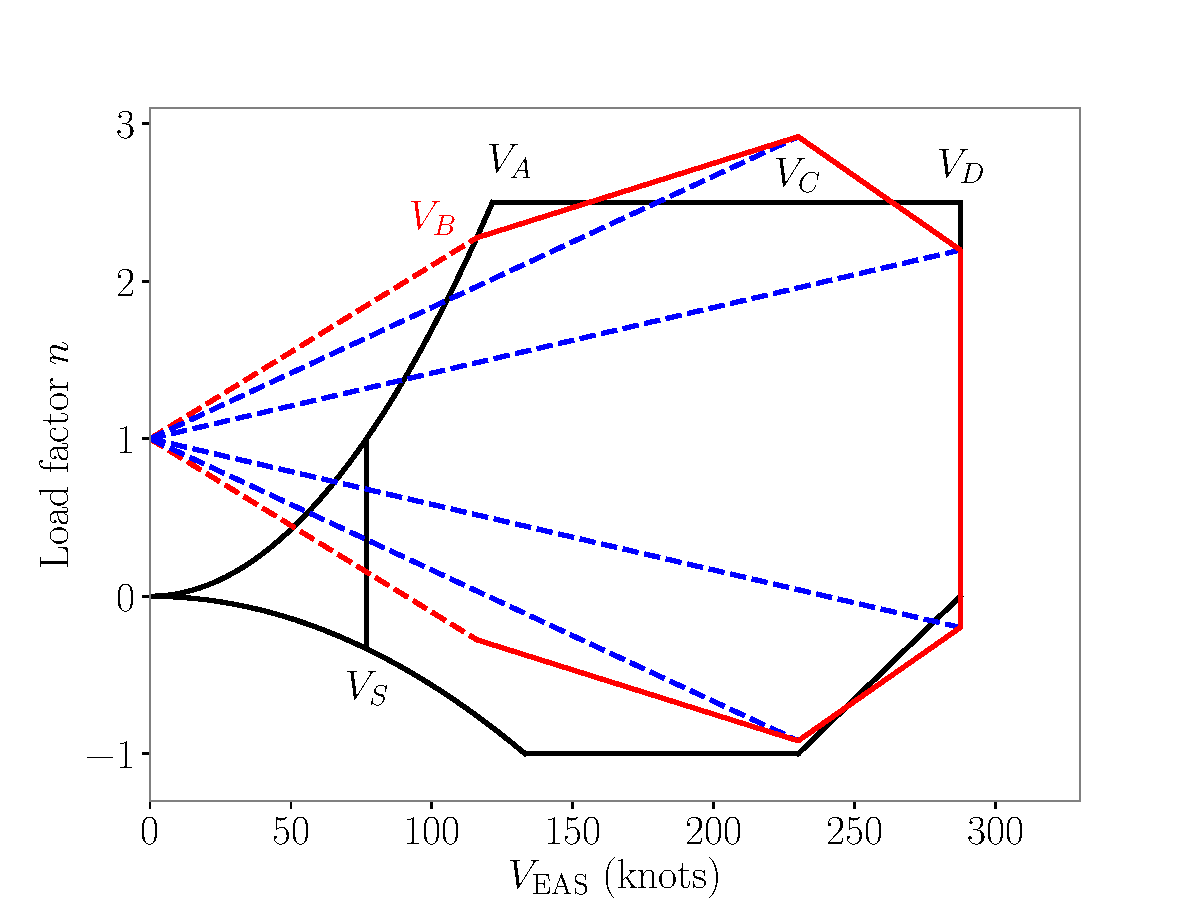
\includegraphics[width=0.6\textwidth]{../Images/v_n_diagram}
 \caption{\textit{V-n} Diagram Used to Determine the Limiting Flight Conditions for the Wing Structure.}
 \label{f:v_n_diagram}
\end{center}
\end{figure}

For the mission performance analyses, the wing model is executed such that it only evaluates the aerodynamic performance without considering the wingbox structure.
Evaluating only the aerodynamics in the mission performance phase is appropriate for two primary reasons. 
First, the aircraft is not expected to experience structurally limiting loads during the nominal mission being evaluated.
Second, although there will undoubtedly be some wing deflection during climb and cruise segments of the flight, this deflection has a negligible effect on the aerodynamic performance. 
Therefore, the wing deflection obtained from the 1g aerostructural analysis completed in the disciplinary design phase was applied to the wing mesh used in the aerodynamics only analysis completed in the mission performance phase.
Given these reasons, removing the structural portion of the analysis was deemed acceptable and thereby enabled a reduction in computational cost during this phase.
% the change in aircraft performance due to changes in wing deflection across the cruise segments of the mission is negligible. 
% The wing deflection obtained from the 1g aerostructural analysis is applied to the wing mesh used in the aero-only cases.
% Nominally, we will not experience structurally limiting loads during the mission, so we subject the wing structure to its limit loads in the discipline design analysis portion.
